\chapter{Design of the System} \label{chap4}
\newpage

\section{Requirement Engineering}
% Apply everything you studied in SE. 

\subsection{Requirement Elicitation}
\justify
Understanding the difficulties students encounter when applying to graduate programs was a requirement elicitation task for MsAdmit. The main needs of the system were determined by analysing past admission records from websites like GradCafe and Edulix, as well as feedback from students and admission counsellors.
To comprehend the elements impacting admissions decisions, current admission platforms and university admission policies were also examined. These results led to the identification of important elements like explainable AI, what-if simulations, application tracking, admission prediction, university recommendations, SOP review, and student profile analysis. A clear and customised admission advice system was developed in accordance with these specifications.
\subsection{Software lifecycle model}


MsAdmit was engineered using the \textbf{Agile Iterative and Incremental Development Model}.  Agile methodology allowed for quick feedback loops to continuously calibrate models and improve user experiences because the platform integrates several technical subsystems, including as machine learning model training, LLM fast engineering, FastAPI microservices, and a reactive frontend.

\begin{itemize}
    \item \textbf{Sprint 1: Data Engineering \& ML Benchmarking:}
    Cleaned and normalized 25,000+ historical admission records. Formulated 25 domain-engineered features, such as \texttt{gpa\_gap}, \texttt{caci\_index}, and \texttt{asymmetric\_gre\_penalty}. Trained baseline models and built the final Stacking Classifier.

    \item \textbf{Sprint 2: Core Backend Architecture \& Authentication:}
    Implemented the FastAPI service skeleton, Pydantic validation schemas, JWT authentication, and database persistence layers using MongoDB Atlas and PostgreSQL.

    \item \textbf{Sprint 3: Semantic Search, LLM Integration \& Document Engine:}
    Embedded 150+ university profiles into a persistent ChromaDB vector store. Developed the eight-criteria prompt pipeline for Google Gemini 1.5 and integrated PyPDF parsing.

    \item \textbf{Sprint 4: Frontend Engineering \& Interactive Components:}
    Built the React 18 and TypeScript frontend using Tailwind CSS. Developed the Applicant Dashboard, Recommendation Cards, TreeSHAP breakdown drawers, and the real time What-If Simulator.

    \item \textbf{Sprint 5: System Integration, Caching \& Performance Hardening:}
    Implemented the dual-mode Redis/in-memory caching service, executed black-box and integration testing suites, and deployed the production stack.
\end{itemize}

\subsection{Requirement Analysis}

The requirements of MsAdmit are classified into functional and non-functional requirements. Functional requirements describe the core features provided by the system, whereas non-functional requirements specify the expected performance, security, usability, and reliability of the system.

\definecolor{headerblue}{RGB}{0,105,165}
\definecolor{lightrow}{RGB}{245,248,251}

% ---------- Table 4.1: Functional Requirements ----------
\subsubsection{Functional Requirements}

\begin{itemize}
    \item \textbf{ Authentication :} Secure user registration, login, and session persistence using JWT tokens with bcrypt password hashing.
    \item \textbf{ Profile Intake (High):} Ingest applicant academic records (GPA, GRE, TOEFL/IELTS, undergrad tier, work experience, publications).
    \item \textbf{Resume Parsing :} Accept PDF resume uploads and extract text using PyPDF to automatically prefill candidate profile metrics.
    \item \textbf{ Admissions ML :} Compute admission competitiveness score across global universities using a trained Stacking Ensemble.
    \item \textbf{ TreeSHAP XAI :} Calculate TreeSHAP feature attributions and return positive and negative factor contributions for each prediction.
    \item \textbf{ Portfolio Engine :} Categorize institutions into balanced 3-3-3 portfolios: Reach (3), Target (3), and Consider (3).
    \item \textbf{Vector Search :} Support natural language semantic queries over the QS Top 150 universities using ChromaDB embeddings.
    \item \textbf{SOP Evaluator :} Critique uploaded SOP drafts against an 8-criteria rubric \cite{mit_sop,cmu_admissions,cmu_sop_guidelines,mit_faculty_essay} using Google Gemini 1.5 with weighted scores.
    \item \textbf{ What-If Engine :} Dynamically re-evaluate admission probabilities in response to interactive parameter adjustments in real time.
    \item \textbf{ App Tracker :} Track shortlisted applications, 6-stage document completion statuses, deadlines, and application fee budgets.
\end{itemize}

\subsubsection{Non-Functional Requirements}

\begin{itemize}
    \item \textbf{ Latency and Speed:} ML inference and SHAP attribution generation must complete within 250\,ms. Cached queries must respond in less than 15\,ms.
    \item \textbf{Accuracy and Loss:} The underlying classification ensemble must achieve ROC-AUC $\geq$ 0.82 and Brier calibration loss $\leq$ 0.18.
    \item \textbf{Security and Authentication:} User credentials are encrypted via salted bcrypt (12 rounds). Protected routes strictly validate JWT Bearer tokens.
    \item \textbf{Fault Tolerance:} Graceful degradation: the system seamlessly fails over to thread-safe in-memory caching and local storage if Redis or Cloudinary is unreachable.
    \item \textbf{Responsiveness:} The user interface is fully responsive, rendering consistently across viewport widths from 320\,px to 2560\,px.
    \item \textbf{ Modularity:} Strict decoupling of API controllers, domain logic, schemas, and persistence models following Clean Architecture.
\end{itemize}


\clearpage
\subsubsection{UML diagrams/ DFDs based on MS-Admit}

\begin{figure}[H]
    \centering
    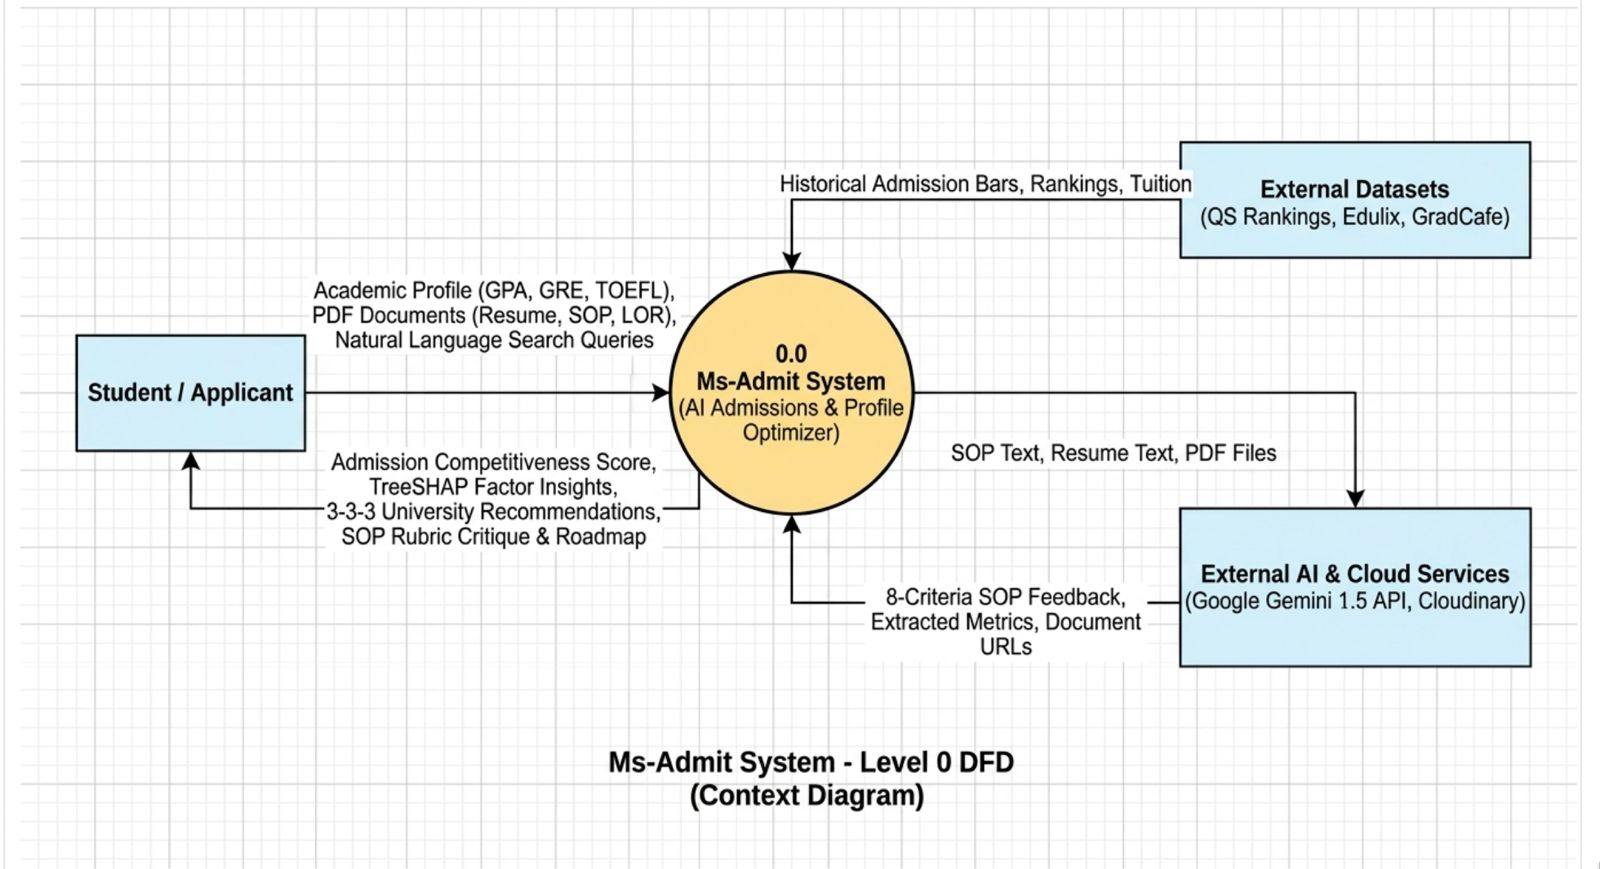
\includegraphics[width=0.85\textwidth]{DFD_0.jpg}
    \caption{DFD Level 0 of MS-Admit}
    \label{fig:dfd_level_0}
\end{figure}
Figure~\ref{fig:dfd_level_0} illustrates the Level 0 Data Flow Diagram (DFD) of MsAdmit, presenting the system's interaction with students, external datasets, and AI services. Students provide their academic profiles, test scores, resumes, SOPs, and search queries as input. The system processes this information using admission prediction models and external AI services to generate competitiveness scores, university recommendations, SOP feedback, and personalized improvement roadmaps. External datasets provide information on university rankings, admission trends, and tuition fees, helping MsAdmit deliver relevant and data-driven guidance to students.
\begin{figure}[H]
    \centering
    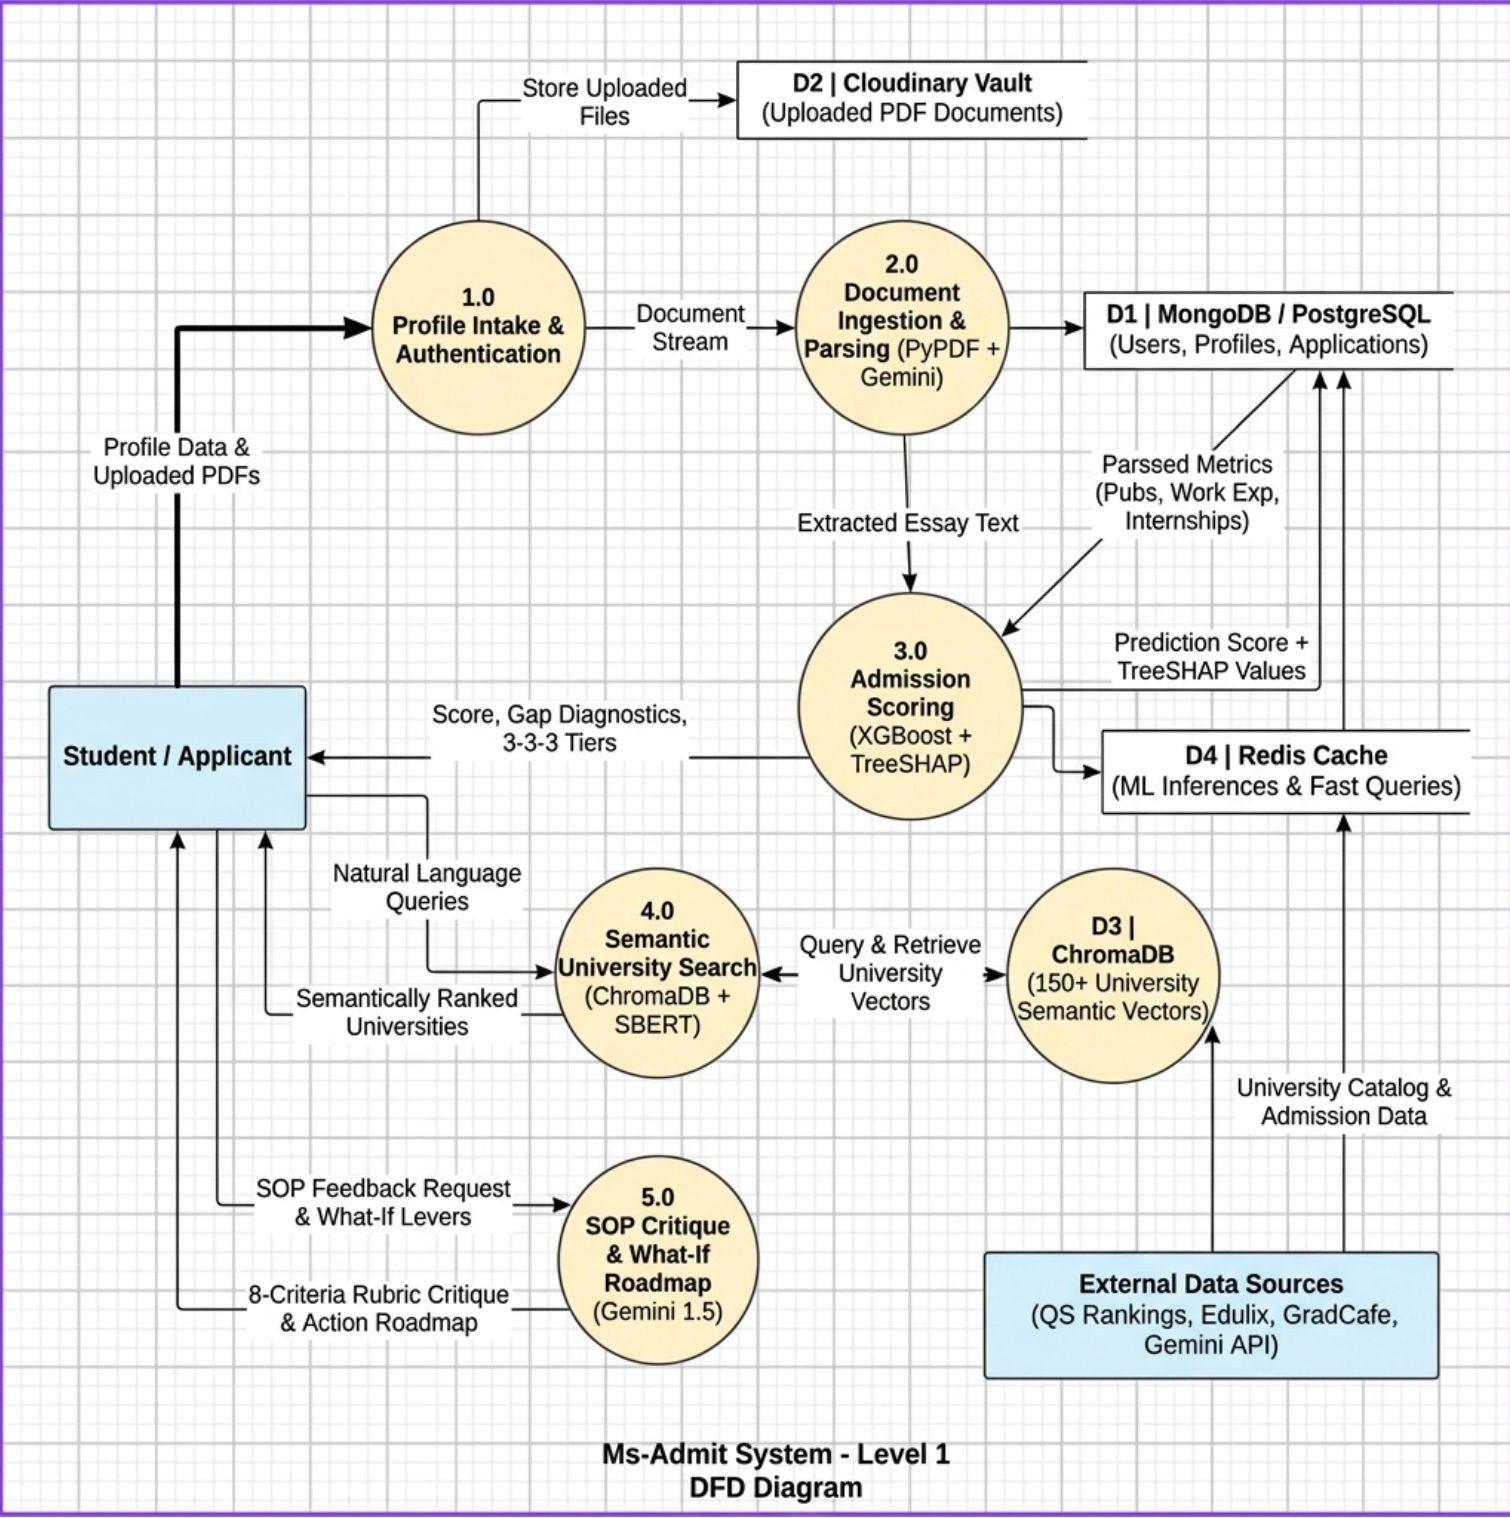
\includegraphics[width=0.85\textwidth]{DFD_1.jpg}
    \caption{DFD Level 1 of MS-Admit}
    \label{fig:dfd_level_1}
\end{figure}
Figure~\ref{fig:dfd_level_1} illustrates the Level 1 Data Flow Diagram (DFD) of MsAdmit, providing a detailed view of its internal processes. The system consists of profile intake and authentication, document ingestion and parsing, admission scoring, semantic university search, and SOP evaluation with a what-if roadmap. These processes interact with databases, caching services, and external data sources to extract relevant information, predict admission competitiveness, recommend suitable universities, and provide personalized feedback to students.
\subsubsection{Cost Analysis}

The operational costs of cloud infrastructure, database services, and external APIs were taken into account while evaluating MsAdmit's economic viability. In order to reduce operational costs while preserving performance and scalability, the system combines premium cloud resources with free-tier services.


%------------------------------------------------
% Estimated Monthly Operational Cost
%------------------------------------------------

\begin{table}[H]
\centering
\caption{Estimated Monthly Operational Cost of MsAdmit}
\label{tab:cost_analysis}
\renewcommand{\arraystretch}{1.3}

\begin{tabularx}{\columnwidth}{|p{2.1cm}|p{2.1cm}|X|p{1.6cm}|}
\hline
\textbf{Service Component} &
\textbf{Provider / Tier} &
\textbf{Operational Purpose} &
\textbf{Monthly Cost} \\
\hline
API Backend Compute &
AWS EC2 t3.medium / Render &
Hosts the FastAPI backend, PDF parsing, and ML inference. &
INR 1,430--2,380 \\
\hline
Frontend Hosting &
Vercel / Netlify &
Hosts and distributes the React frontend. &
INR 0 (Free Tier) \\
\hline
Database &
MongoDB Atlas &
Stores user profiles, prediction results, and application data. &
Depends on usage / free tier \\
\hline
Vector Database &
ChromaDB &
Stores university embeddings for semantic search. &
Included in backend hosting \\
\hline
Caching Service &
Redis Cloud / In-memory Cache &
Improves response time for repeated requests. &
INR 0--950 (estimated) \\
\hline
External LLM API &
Google Gemini 1.5 &
Evaluates SOPs and generates feedback. &
Depends on API usage \\
\hline
Document Storage &
Cloudinary &
Stores uploaded resumes and related documents. &
Depends on usage / free tier \\
\hline
\end{tabularx}
\end{table}

\noindent
 Table 4.1 shows the  estimated monthly
operational costs of MsAdmit and supports its financial feasibility.
The use of free-tier services and scalable infrastructure helps
minimize initial expenses, making the system practical to implement
and maintain. Although costs may increase with user activity and
AI API usage, selecting suitable service plans and optimizing
resource utilization can help ensure the platform remains
cost-effective and sustainable in the long term.


% --- document ---


\clearpage
\subsubsection{Hardware and software requirements}



\begin{table}[H]
\centering
\caption{Hardware Requirements for MsAdmit}
\label{tab:hardware_requirements}

\large
\renewcommand{\arraystretch}{1.8}
\setlength{\tabcolsep}{8pt}

\begin{tabularx}{\textwidth}{
|>{\raggedright\arraybackslash}p{3.2cm}
|>{\raggedright\arraybackslash}p{3.2cm}
|>{\raggedright\arraybackslash}p{3.2cm}
|X|}
\hline
\textbf{Component} &
\textbf{Minimum Requirement} &
\textbf{Recommended Requirement} &
\textbf{Purpose} \\
\hline

Processor &
Intel Core i3 or equivalent &
Intel Core i5 or equivalent &
Runs the application and development tools. \\
\hline

RAM &
8 GB &
16 GB or more &
Supports backend services, database operations, and development tools. \\
\hline

Storage &
10 GB free space &
20 GB or more free space &
Stores source code, dependencies, datasets, and project files. \\
\hline

Internet Connection &
Stable broadband connection &
High-speed broadband connection &
Enables API access, cloud services, and university data retrieval. \\
\hline
\end{tabularx}
\end{table}

\justify
The Table 4.2 shows hardware requirements for MsAdmit includes a suitable processor, sufficient RAM, adequate storage, a display, and a stable internet connection. These resources support application development, database operations, machine learning tasks, and access to external AI services. The recommended specifications help ensure smooth execution of the system and efficient performance during development and testing.


\begin{table}[H]
\centering
\caption{Software Requirements for MsAdmit}
\label{tab:software_requirements}
\renewcommand{\arraystretch}{1.3}
\begin{tabularx}{\textwidth}{
|>{\raggedright\arraybackslash}p{3cm}
|>{\raggedright\arraybackslash}p{3cm}
|>{\raggedright\arraybackslash}p{3cm}
|X|}
\hline
\textbf{Software / Technology} &
\textbf{Version / Platform} &
\textbf{Category} &
\textbf{Purpose} \\
\hline
Python &
3.10 or compatible &
Programming Language &
Implements the backend, data processing, and machine learning components. \\
\hline
FastAPI &
Compatible version &
Backend Framework &
Provides APIs for profile evaluation and system functionality. \\
\hline
Next.js &
Compatible version &
Frontend Framework &
Develops the user interface and interactive application pages. \\
\hline
MongoDB Atlas &
Cloud-based &
Database &
Stores user profiles, prediction results, and application information. \\
\hline
XGBoost &
Compatible version &
Machine Learning &
Predicts admission competitiveness using applicant profile data. \\
\hline
SHAP &
Compatible version &
Explainable AI &
Explains the factors influencing model predictions. \\
\hline
ChromaDB &
Compatible version &
Vector Database &
Supports semantic search using university data embeddings. \\
\hline
Redis &
Compatible version &
Caching &
Improves response times by caching frequently accessed data. \\
\hline
Google Gemini API &
API-based service &
Generative AI &
Supports SOP evaluation and feedback generation. \\
\hline
Visual Studio Code &
Compatible version &
Development Environment &
Provides an environment for writing and debugging code. \\
\hline
Git and GitHub &
Web-based / compatible version &
Version Control &
Tracks code changes and supports collaborative development. \\
\hline
Web Browser &
Chrome, Firefox, or Safari &
Application Access &
Allows users to access the MsAdmit web application. \\
\hline
\end{tabularx}
\end{table}
\justify
The Table 4.3 shows software requirements for MsAdmit includes the technologies needed to develop and operate the system. Python, FastAPI, and Next.js support backend and frontend development, while MongoDB manages data storage. XGBoost and SHAP enable admission predictions and explainability, and ChromaDB supports semantic university searches. Redis provides caching, while the Gemini API assists with SOP evaluation and feedback generation. Together, these technologies ensure efficient system functionality and personalized admission guidance.

\section{System architecture}



\subsection{UI/UX Diagram}

\begin{figure}[!htbp]
    \centering
    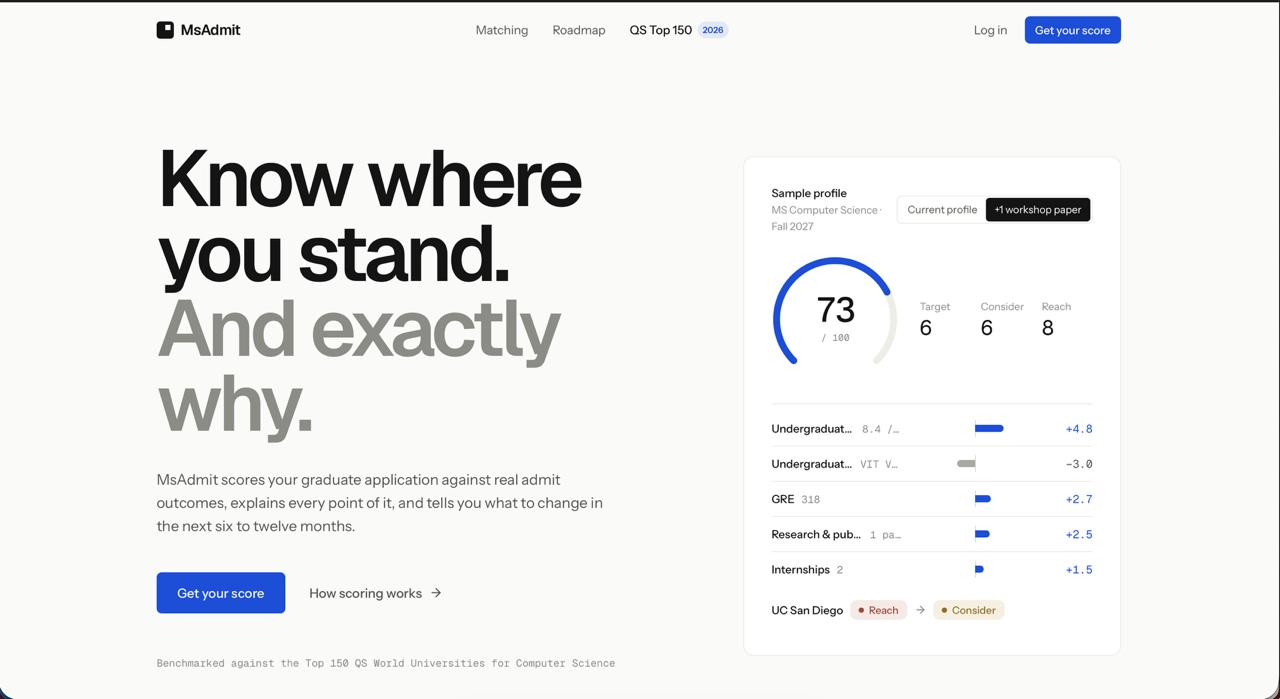
\includegraphics[width=0.85\textwidth]{uiux.jpeg}
    \caption{UI/UX Diagram of MsAdmit}
    \label{fig:uiux}
\end{figure}

\noindent
Figure \ref{fig:uiux} illustrates the homepage of MsAdmit, 
featuring a clean interface, university matching, personalized 
improvement roadmaps, and university rankings. The dashboard 
displays the admission competitiveness score and factors 
influencing the student's profile.



\subsection{Block Diagram}

\begin{figure}[!htbp]
    \centering
    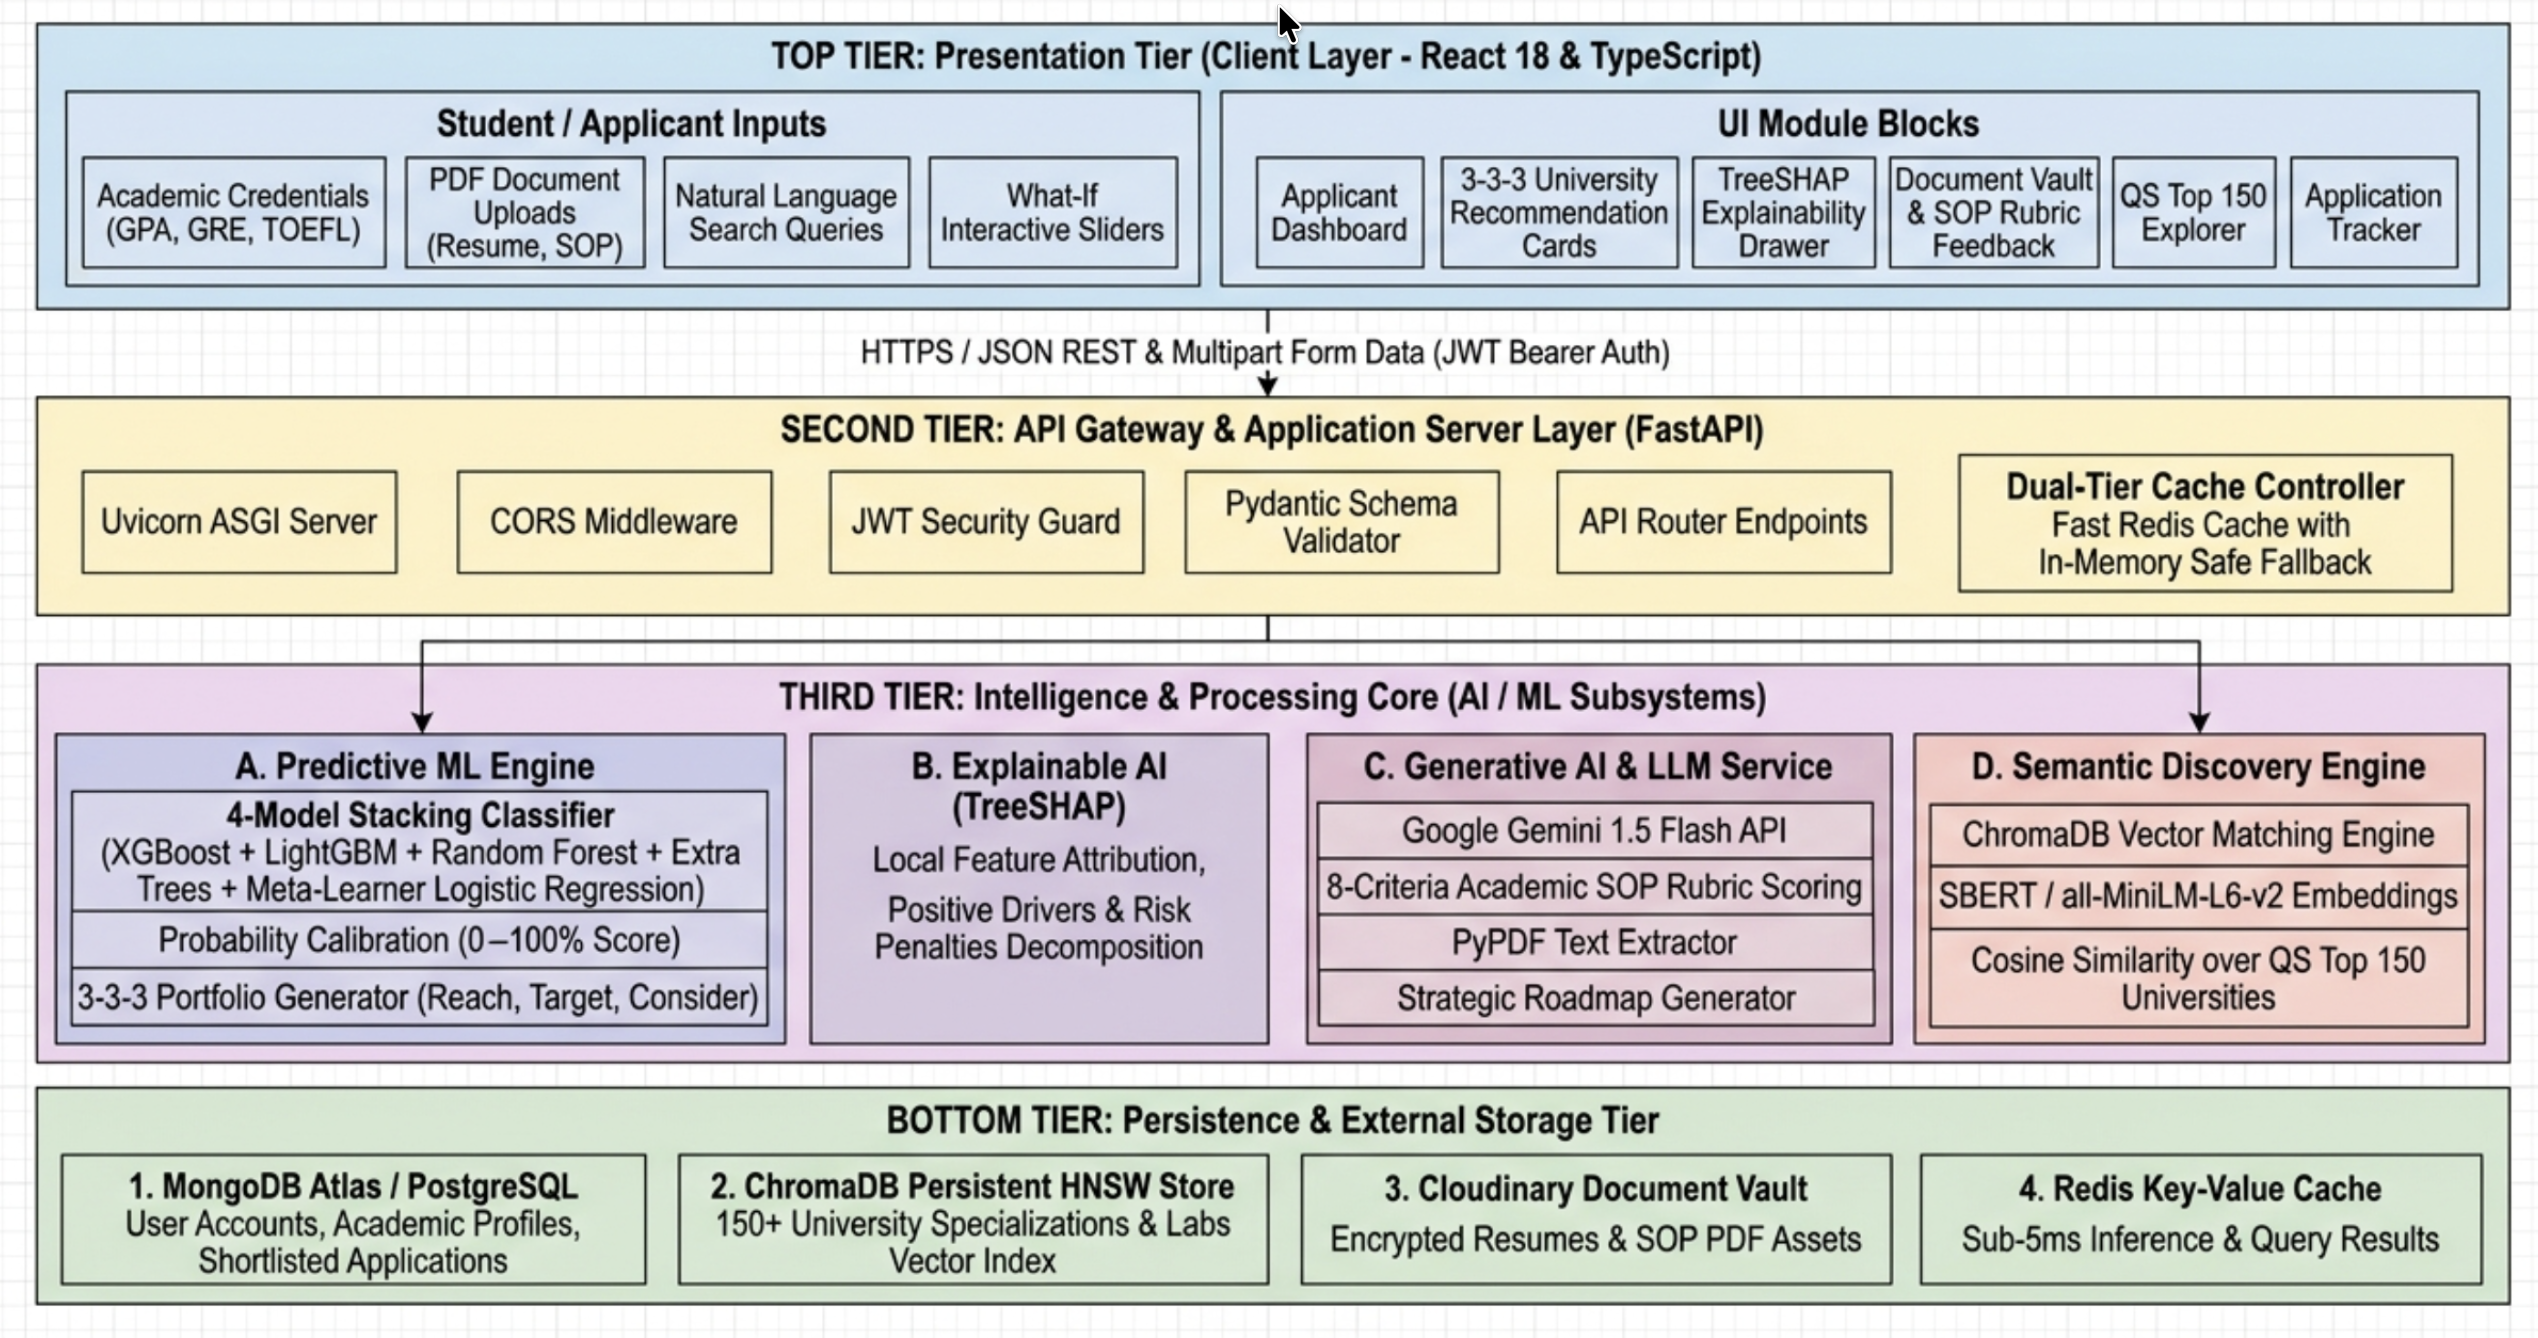
\includegraphics[width=0.95\textwidth]{Screenshot 2026-10-27 at 3.10.37 PM.png}
    \caption{Block Diagram of MsAdmit}
    \label{fig:blockdiagram}
\end{figure}

\newpage
\justify
Figure \ref{fig:blockdiagram}illustrates the overall system architecture of MsAdmit, showing the interaction between the presentation layer, API gateway, AI/ML processing core, and persistence and external storage layer. These components work together to predict admission probabilities, explain model predictions, evaluate Statements of Purpose (SOPs), recommend suitable universities, and manage applicant profiles and application data.


\justify
This chapter presented the system design of MsAdmit, covering requirement engineering, the software development lifecycle, functional and non-functional requirements, cost analysis, and hardware and software requirements. It also described the system architecture, data flow diagrams, and UI/UX design, explaining how the different components work together to provide admission prediction, university recommendations, SOP evaluation, and personalized guidance.
